% %% ==============================
% Part is used only in PhD thesis
\part{The ideas}
\chapter{\iflanguage{ngerman}{Methoden}{Methode and Pipeline Design}}
\label{sec:Pipeline}
%% ==============================
The remainder of this section describes the specific domain randomization and neural network training methodology we use. And we will walk through the pipeline and explain how different modules interact with each other. Firstly an overview of the pipeline architecture is presented, and the functionality of different modules will be introduced. Then the pipeline about the construction and training of neural network model will be described. Lastly the details of evaluation methods are given.


\section{Pipeline Architecture}
Given some objects of interest ${s_i}_i$, our goal is to train an object detector $d(I_0)$ that maps a single camera frame $I_0$ to the Cartesian coordinates ${(x_i, y_i, \theta_i)}_i$ of each object. In addition to the objects of interest, our scenes sometimes contain distractor objects that must be ignored by the network. Our approach is to train a deep neural network in simulation using domain randomization. 

The entire pipleline consists of four parts, namely the simulation environment module, the model training module, the real world module and the evaluation module. The simulation environment is built based on unity3D and is used to generate simulation data needed for model training. The model training module is used to preprocess the training data, then build and train the CNN model. The acquisition of real data is implemented in the real world module, and the prediction effect of them model trained by pure simulation data can be evaluated by real data. The evaluation module can be used to analyze the performance of the model on simulation data, and can also be used to analyze the performance in the real world, that is, the CNN model trained on the simulation data predicts the 3D pose of real world image and identifies error between the actual pose of the object. The structure of the entire pipeline is shown in figure 4.1. The final goal is to achieve better object recognition and detection accuracy by adjusting the structure of the CNN model and the rendering effect of the simulation environment.
\begin{figure}[h]
	\includegraphics[width=0.9\textwidth]{Figures/Section4_Pipeline_structure.pdf} 
	\centering
	\captionsetup{justification=centering}
	\caption{Pipeline Structure}
	\label{fig:pipeline}
\end{figure}

\section{Domain randomization in Unity3D}
The purpose of domain randomization is to provide enough simulated variability at training time such that at test time the model is able to generalize to real-world data. We randomize the following aspects of the domain for each sample used during training:
\begin{itemize}
	\item Number and shape of distractor objects on the table
	\item Position and texture of all objects on the table
	\item Textures of the table, floor, skybox, and robot
	\item Position, orientation, and field of view of the camera
	\item Number of lights in the scene
	\item Position, orientation, and specular characteristics of the lights
	\item Type and amount of random noise added to image
\end{itemize}
Since we use monocular camera image from an uncalibrated camera to estimate object positions, we fix the height of the table in simulation, effectively creating a 3D pose estimation task. Random textures are chosen among the following:
\begin{itemize}
	\item A random RGB value
	\item Additional pattern
\end{itemize}
The textures of all objects are chosen uniformly at random – the detector does not have access to the color of the object(s) of interest at training time, only their size and shape. We render images using the Unity3D’s \cite{bartneck2015robot} built-in renderer. This renderer is not intended to be photo-realistic, and physically plausible choices of textures and lighting are not needed.

Between 0 and 10 distractor objects are added to the table in each scene. Distractor objects on the floor or in the background are unnecessary, despite some clutter (e.g., cables) on the floor in our real images.

Our method avoids calibration and precise placement of the camera in the real world by randomizing characteristics of the cameras used to render images in training. We manually place a camera in the simulated scene that approximately matches the viewpoint and field of view of the real camera. Each training sample places the camera randomly within a (10 × 5 × 10) cm box around this initial point. The viewing angle of the camera is calculated analytically to point at a fixed point on the table, and then offset by up to 0.1 radians in each direction. The field of view is also scaled by up to 5 \% from the starting point.

According to the previous introduction, the purpose of the whole experiment is to explore the performance of of the CNN model trained by pure simulation data and how to improve the recognition accuracy and ability of the model by  adjusting the model structure and parameters and changing the rendering effect in the simulation environment. Therefore, the construction of the simulation environment is a very important part of the experiment. We require that the simulation environment have the following basic characteristics:
\begin{enumerate}
	\item The rendering effect can be modified in real time, because the training of the CNN model relies on a large amount of training data, so in the data generation process, in order to obtain images with different rendering effects to fit the changes of the environmental parameters in the real world, the rendering must be able to be modified in real time during the image data generation process.
	\item The positional parameters of target objects in the simulation environment are variable in real time. Since the purpose of the experiment is to predict the 3D pose of the target object, the simulation data needs to be contain a large amount of different pose information in the simulation scene for training the CNN model. Therefore the CNN model can learn a lot of different information, which is beneficial to the generalization effect of the model, so as to get better performance in the real word.
	\item The environment need to generate the pose information of the object. As a supervised learning model, the CNN model requires effective label data by each image data for model training. In the process of collecting real world data, the labeling task for each image is very cumbersome and time-consuming, which often requires a lot of manpower. In order to solve this problem, the simulation environment should include the 3D pose information corresponding to the target object of each sample, and the label information can be directly output corresponding to the image.
\end{enumerate}
Based on the above requirements, we chose Unity3D as the rendering engine for the simulation environment. As described in section 3, Unity3D is a commercial game engine with good user interface that is easy for operators to render and model. The graphics rendering engine of Unity3D can meet the requirements of image rendering task in our experiment. At the same time, Unity3D has a rich set of advanced APIs.   By pre-writing script code, we can achieve the required rendering effects and settings.


\subsection{Scene Construction}
This step can be done directly in the graphical interface window of Unity3D. First we need to import the model into the scene, it can be generated in other modeling software and then imported into Unity3D, or we can directly generate a simple geometry model in Unity. Then other components in the scene need to be added, such as cameras, different light sources, and environmental components. The entire scene is built similar to the modeling process in general modeling software. After all required scene components have successfully appeared, we can adjust the relative positional relationship of components to generate the desired scene. A completed simulation scenario is shown in figure 4.2. After the scene is built, the next step is to implement the required functionality through different functional module written in scripts. 
\begin{figure}[h]
	\includegraphics[width=0.7\textwidth]{Figures/Section4_Scene.png} 
	\centering
	\captionsetup{justification=centering}
	\caption{An example of Simulation Scene}
	\label{fig:simulation_scene}
\end{figure}

\subsection{Object Randomization Module}
As mentioned before, in order to make the rendered objects have different rendering effects, and randomly generate and output different pose in a certain area, we have written the function module in script called object randomization module. 

\textbf{The main function}:
\begin{enumerate}
	\item Select the target object that appears in the scene and randomly generate interfering objects in each sample
	\item Randomly render the color and texture of the object appearing in the image
	\item Randomly generate the pose of target and interfering objects, and record the pose information in each sample  
\end{enumerate}

\textbf{Function details}:

First, some basic parameters will be set, eg. data output address, the number of images to be generated. And the target object and the interfering objects need to be selected from the candidate objects list. After all the basic parameters have been read in, the program begins to prepare to render the image frame by frame. The program randomly determines the number of objects that appear in the frame of frame, including the target object and the interfering object. When the number of objects of current frame image is determined, the individual objects are rendered one by one. Firstly for the target object, it's pose and texture will be randomly generated. After that, the interfering objects will be rendered under the conditions that avoid collision with previously generated objects. When all the objects in current frame have been rendered, the pose information of target object will be stored. Next, it is judged whether the preset number of images is reached, if the number of image is not reached, the rendering process is continued in a loop. If all the images have been rendered, the rendering loop will be terminated and the pose information of target object of each frame will be packed into .json\footnote{JSON (JavaScript Object Notation): https://www.json.org/} file and output. As shown in figure 4.3, the function of the object randomization module is implemented by looping. After each re-entry loop, the new image will be randomly rendered, at the same time, the pose information corresponding to current frame will be stored.

\begin{figure}[h]
	\includegraphics[width=0.9\textwidth]{Figures/Section4_Object_randomization.pdf} 
	\centering
	\captionsetup{justification=centering}
	\caption{Object Randomization Module}
	\label{fig:objrand}
\end{figure}

\textbf{APIs Summary:}
\begin{enumerate}
	\item Target selector: Select the target object from the candidate objects
	\item Interfering option: Select whether the interfering objects appear or not
	\item Texture option: Select whether to add extra texture to the target object, or perform solid color rendering on the target object
	\item Target color option: Select the HSV color rendering range of the target object, it can be selected to render the object around actual color or render full randomly
\end{enumerate}
All APIs are integrated into the Unity3D user interface via scripts, which can be selected directly via input column or down menu, and the functionality of the APIs can be further extended according to requirements to achieve different functional combinations. Figure 4.4 shows what the currently written APIs look like in the Unity3D control panel.
\begin{figure}[h]
	\includegraphics[width=0.5\textwidth]{Figures/Section4_ObjrandApi.png} 
	\centering
	\captionsetup{justification=centering}
	\caption{APIs for Object Randomization Module}
	\label{fig:objrandapi}
\end{figure}

\subsection{Environment Randomization Module}
According to the method of domain randomization, in addition to the random rendering of target object and the interfering objects in the scene, it is necessary to randomly render the environment of the entire scene. In our experiments, the scene mainly include the floor, table, robot, ambient light and the skybox.

\textbf{The main function:}
\begin{enumerate}
	\item Randomly render the floor, table, skybox
	\item Randomly render the ambient light with different numbers, lighting angles and spectrum
\end{enumerate}

\textbf{Function details:}

The environment of the scene mainly includes the floor, table, ambient light and skybox. The program first determines the environmental objects in scene and associates them with the objects defined in scripts. Then according to the setting parameters to determine whether the environment object is rendered with additional complex textures, otherwise it will be randomly rendered with a solid color. After that, the ambient light source in the scene will be rendered. The light source is mainly divided into directional light and point light. The directional light is the main light source in the environment, it is used to simulate the sunlight or the main illumination source in the real world. The number of the directional light and the lighting angle will be randomly rendered. The spectrum of directional light can be selected as daylight or full randomly color. Finally, the number and location of point light are randomly rendered, which is used to simulate the effects of reflected light in the real world. Figure 4.5 describes the implementation of environment randomization.
\begin{figure}[h]
	\includegraphics[width=0.9\textwidth]{Figures/Section4_Environment_randomization.pdf} 
	\centering
	\captionsetup{justification=centering}
	\caption{Environment Randomization Module}
	\label{fig:envrd}
\end{figure}

\textbf{Api summary:}
\begin{enumerate}
	\item Texture option: Whether to render environment with additional complex texture, or with solid color
	\item Num of directional light: Determine the number of directional light added to the scene
	\item Spectrum option: Select the spectrum of the light source, which can be selected to simulate daylight or render on full random color
	\item Num of point light: Determine the number of point lights in the scene 
\end{enumerate}

APIs are also integrated into the Unity3D interface through the setup script, as shown in figure 4.6.
\begin{figure}[h]
	\includegraphics[width=0.5\textwidth]{Figures/Section4_EnvrdApi.png} 
	\centering
	\captionsetup{justification=centering}
	\caption{APIs for Environment Randomization Module}
	\label{fig:envrdApi}
\end{figure}

\subsection{Camera Randomization Module}
In the scene rendering process, the image data we need is obtained from the perspective of the scene camera, so we need special camera function module to control the position and direction of the camera angle to simulate the pose of the camera in real world. The parameters of the camera mainly include external parameters and internal parameters. The external parameters describes the positional relationship of the camera coordinate system with respect to the word coordinate system, while the internal parameters describes the transformation between image plane coordinates and pixel coordinates, and also the geometric distortion introduced by the optics. \cite{zhang2000flexible}. Due to the certain error in the installation of the camera and in the internal structure, camera calibration is often required before using it in the real world. For camera calibration Zhang' s method can be used. For our experiment this error will cause a certain deviation between the simulated image and the real world image. In order to avoid the camera calibration caused from this error, we will randomize the characteristics of the camera in the rendering process.

\textbf{The main function:}
\begin{enumerate}
	\item Place the camera with a initial pose and start it with default initial parameters, which include focus length and field of view (FoV).
	\item In each frame randomize the camera' s position in a small range of area and also the viewing angle and FoV.
	\item Control the camera to save the image after each frame is rendered
\end{enumerate}

\textbf{Function details:}

The camera' s initial position and parameters will be read in, then the camera can be set by script to match the state of the camera in real world. In each sample, the camera is randomly moved in a predetermined small box area, which is placed around the initial position of the camera. After that setting the view angle of camera point to the center of the table analytically, and then a deflection will be set in each direction. The camera' s FoV will be randomly scaled in a small range. After completing the randomization of camera, the image storage process will wait until the rendering process is complete. The entire process is shown in figure 4.7.
\begin{figure}[h]
	\includegraphics[width=0.9\textwidth]{Figures/Section4_Camera_randomization.pdf} 
	\centering
	\captionsetup{justification=centering}
	\caption{Camera Randomization Module}
	\label{fig:camrand}
\end{figure}

\textbf{Api summary}
\begin{enumerate}
	\item Initial Pose: Set the initial pose of camera
	\item Max Placement Error: Set the maximum random translation error range in the x, y, z directions. That is, the box area around the initial point mentioned before.
	\item Max Angle Error: Set the maximum deflection error range of the view angle to simulate the error caused by installation.
	\item Enable Second Camera: Whether enable second camera or not.
\end{enumerate}
The APIs is integrated into the Unity3D control panel, as shown in figure 4.8.
\begin{figure}[h]
	\includegraphics[width=0.5\textwidth]{Figures/Section4_CamerardApi.png} 
	\centering
	\captionsetup{justification=centering}
	\caption{APIs for Camera Randomization Module}
	\label{fig:camrandApi}
\end{figure}


\subsection{Robot-arm Randomization Module}
The robot arm in the simulation scene can be set with a random grab gesture to fit the occlusion on the view area during the capture process in real world. Depending on  the requirement , we can select whether the robot arm randomly generates the grab gesture or keep in the initial state during the rendering process.

\textbf{The main function:}
\begin{enumerate}
	\item Control the angle of each joint of the robot arm to randomly generate different grab gesture.
\end{enumerate}
Figure 4.9 shows the effect of the robot arm in different grab gesture.
\begin{figure}[h]
	\includegraphics[width=0.9\textwidth]{Figures/Section4_Robotarm.png} 
	\centering
	\captionsetup{justification=centering}
	\caption{Different grab gestures of robot arm}
	\label{fig:robotarm}
\end{figure}

\subsection{Common Setting Module}
Some basic globe parameters can be entered manually directly through the parameters setting module, or read from a pre-written XML file.

\textbf{The main function:}
\begin{enumerate}
	\item Read in global parameters which are manually entered
	\item Read the parameters from the XML file
\end{enumerate}

\begin{figure}[h]
	\includegraphics[width=0.5\textwidth]{Figures/Section4_CommonApi.png} 
	\centering
	\captionsetup{justification=centering}
	\caption{APIs for Common Setting Module}
	\label{fig:commonapi}
\end{figure}

\textbf{Api summary:}
\begin{enumerate}
	\item Parameter entry: manually enter the global parameter, or read in from the xml 
	\item Manually entered parameter content (storage address, picture resolution)
	\item Total Num of Images: set the number of  images to be rendered
	\item Enable save images: Whether save images or not 
\end{enumerate}


\section{Model architecture and training}
Based on the simulation environment introduced in the previous section, we obtained a large number of image data with labels. Each sample is randomly rendered based on domain randomization through the unity engine. The next step is to use the simulation data to train the CNN model. In this Section, the Setup of the model structure and the training process of it will be introduced. 

\subsection{Environment set up}
Keras \footnote{https://keras.io/} is the recommended library for beginners, since its learning curve is very smooth compared to others, and at the moment it is one of the popular middleware to implement neural networks. Keras is a Python \footnote{https://www.python.org/} library that provides, in a simple way, the creation of a wide range of Deep Learning models using as backend other libraries such as TensorFlow \footnote{https://www.tensorflow.org/}, Theano \footnote{http://deeplearning.net/software/theano/} or CNTK \footnote{https://github.com/Microsoft/CNTK}. It was developed and maintained by François Chollet, an engineer from Google, and his code has been released under the permissive license of MIT. Also an important thing is that Keras is included in TensorFlow as a API. Although Keras is currently included in Tensorflow package, but can also be used as a Python library. 

Our model training environment is based on Keras, because Keras provides a number of advanced APIs that make it easy for us to build CNN models quickly and modify the structure of the model. From Keras we can directly import many popular networks with good performance in the field of computer vision, such as VGG-net, Resnet. At the same time, Keras provides an interface that can import pre-trained weights of these neural networks based on ImageNet \footnote{http://www.image-net.org/}, so we can import the models with the initial weights, and then modify the structure of the neural network by modifying the fully connected layers and output layer to get the model we want. This enable us to implement fast experiments to doing good research.

\subsection{Data Preprocess and import}
For the training of the neural network model, the first step is the preprocessing and import of training data. Since the data obtained from Unity3D are separate images und a file in json format which has stored label information. If the training data are directly read into the neural network, the image data need to be processed in real time, which will greatly consume the GPU and CPU resources of system. In this case the training efficiency will be reduced. So we need to preprocess and manage the large amounts of training data, which is very import for the training efficiency.

\textbf{The Hierarchical Data Format(HDF5)}

The first thing we need to do is to convert the training data that was stored in raw-image format into an array-like format, which can be read directly by the neural network model. Here HDF5 is chosen to store the image data, because it has good hierarchical structures for data storage, and data are stored in an array-like form.

The Hierarchical Data Format version 5 (HDF5) \footnote{https://www.hdfgroup.org/solutions/hdf5/} is a popular format for storing and exchanging unstructured data such as images, videos or volumes in raw format for use in various areas of research or development. It is supported by many programming languages and APIs and is therefore becoming increasingly popular. This also applies to storing data for use in machine learning workflows.

A HDF5 file consists of two major types of objects: Datasets and groups. Datasets are multidimensional arrays of a homogeneous type such as 8-bit unsigned integer or 32-bit floating point numbers. Groups on the other hand are hierarchical structures designed for holding datasets or other groups, building a file system-like hierarchy of datasets. Additionally, groups and datasets might have metadata in the form of user-defined attributes attached to them. Python supports the HDF5 format using the h5py package. This package wraps the native HDF C API and supports almost the full functionality of the format, including reading and writing HDF5 files.

\textbf{Image Preprocessing}

The format of the image data obtained from the Unity3D is JPG (Joint Photographic Experts Group) \footnote{https://jpeg.org/about.html} with a default resolution of $640\times480$. The default input size of the CNN model is $224\times224\times3$, where 224 represent the length and width of the image. Because we use color image, each image data will have 3 channels to store the r,g,b values. Therefore, we need tor resize the image and store it in the array-like form, and store the label information corresponding to each image. Here we use the dataset and group methods to classify the different type of data for storage.

We classify the dataset into 2 groups, image and label. By creating different groups, the image data and the label data are respectively written into each group in array-like form. In each group, the corresponding entire data will form a whole dataset. For example, there are N images and labels in the dataset, which are jpg format with a resolution of $640\times480$. After importing the images and labels into the HDF5 file we get two groups of dataset, image and label. In the image group, the shape of dataset is $N\times224\times224\times3$. Which means the image data are downsized to $224\times224$, and in the dataset exist N images. Meanwhile the size of the dataset in label group is $N\times3$, because each label corresponds to the image has 3 label information, which are position coordinate along the axis x and y, and the rotation $\theta$ around the z axis. In this way, by storing the image in HDF5 file, we get the array-like dataset. Figure 4.24 shows a example of the data structure in HDF5 file. Next we will design how to read the data into the training model.

\begin{figure}[h]
	\includegraphics[width=0.8\textwidth]{Figures/Section4_HDF.png} 
	\centering
	\caption{An example of a hdf5 file with  three groups, including images, image\_2 and labels. The size of the dataset in images is $ 100000 \times224 \times 224 \times3 $, which means 100000 RGB images with size of $224\times 224$ are stored in the dataset.}
	\label{fig:hdf}
\end{figure}


\textbf{Data Import}
For the training of CNN models, mini-batch training \cite{li2014efficient} will be used. As mentioned in Chapter 2, mini-batch training allows for a more robust convergence and helps avoid local minima. The batched updates provide a computationally more efficient process than stochastic gradient descent, which benefits from vectorization. Not only that, the batching allows both the efficiency of not having all training data in memory and algorithm implementations, which fits in the memory easily.

In this case, we use data generator to get the batch training data from the dataset. The generator is run in parallel to the model for efficiency. Through the generator the number of data obtained from the dataset can be controlled by giving the batch size parameter. That means the training process can be implemented under different batch sizes, and through experiment we can choose a batch size to achieve faster convergence speed.


\subsection{Architecture design}

we parametrize our object detector with a deep convolutional neural network. As mentioned in the previous chapters, several well-known CNN models such as VGG-16 \cite{simonyan2014very}, ResNet50 \cite{he2016deep}, Inception V3 \cite{szegedy2016rethinking}, have very good performance on the variable computer vision tasks. Similar to the work in \cite{tobin2017domain}, in our experiment we will use the modified version the these models. By retaining the convolutional layers of the model, but modifying the structure of the fully connected layers, a new model can be established. Like \cite{tobin2017domain} dropout will be removed from the model.  Figure 4 shows a modified VGG-16 model by modifying its fully connected layers. In this model, ReLU nonlinearities are used in each convolutional layers. And we reduce the size of the fully connected layer to 256 and 64, and modify the output layer to 3 outputs, which predict the 3D pose of the object of interest.

\begin{figure}[h]
	\includegraphics[width=0.8\textwidth]{Figures/Section4_vgg16.png} 
	\centering
	\caption{The initial model architecture of VGG-16. Each vertical bar corresponds to a layer of the model. ReLU nonlinearities are used throughout, and max pooling occurs between each of the groupings of convolutional layers. The input is an image from an external webcam downsized to (224 × 224) and the output of the network predicts the (x, y, $\theta$) coordinates of object(s) of interest.}
	\label{fig:vgg161}
\end{figure}

Similar to the model above, the modified ResNet50 model and Inception V3 model are shown in figure 4. In the experiment, the performance of each model will be verified, the goal is to select the model with best performance and this model will be used to verify the impact of different rendering conditions. Finally, we the improve the recognition accuracy in the real world by analyzing the optimal rendering conditions and model structure.

\begin{figure}[h]
	\includegraphics[width=0.8\textwidth]{Figures/Section4_inceptionv3.png} 
	\centering
	\caption{The initial model architecture of Inception-v3. Each vertical bar corresponds to a layer or module of the model. The input is an image from an external webcam downsized to (224 × 224) and the output of the network predicts the (x, y, $\theta$) coordinates of object(s) of interest.}
	\label{fig:inceptionv3}
\end{figure}

\subsection{Multicamera system}
Once we have a single-image object detector, we can combine their outputs to obtain improved detection performance. Roughly speaking, if we receive multiple observations of the same scene but from different angles, then even if these observations are correlated it is quite possible that the combined beliefs derived from all of the observations will be better than any single observation\cite{coates2010multi}. 


In our setting, we assume that we are given multiple different images of the same scene where the viewpoints from which the images were captured are separated by a modest baseline (similar to what could be achieved with multiple cameras on a robot, or by a robot that can move itself or the cameras a short distance). We’ll assume from now on that we have just two cameras, but the same technique can straight-forwardly be applied to any number of observations.

For the multi-cam system, since there are two image as input data of the training model in each frame, we use two convolutional layer models in parallel to process the input data. That means two models learn the information of the two image at the same time. After the convolutional layers, the two model are fed to a fully connected layer to fuse the information from the two images. A example of the model is shown in figure 4, in the model all layers use ReLU \cite{nair2010rectified} activation function. The 3 outputs in the last layer predict the 3D of target object.

\subsection{Model training}
\textbf{Loss function}
The final output of our model are position and rotation, which includes two different units, one of them is the length unit of the position prediction, and the other is the angle unit for predicting the rotation. For each part of prediction L2 loss will be used, that means there are two Loss $L(x,y)$, $L(\theta)$ here, corresponding to position and rotation. Since the units of the two Loss function are different, for a better training effect we use a coefficient to correct the $L(\theta)$. The formula is as follow:
\begin{equation}
	L(total)=L(x,y)+Coef*L(\theta)
\end{equation}

\textbf{Optimization}  
Gradient descent is on of the most popular algorithms to perform optimization and by far the most common way to optimize neural networks. As we mentioned in the previous section, there are 3 variants of gradient descent, which differ in how much data we use to compute the gradient of the loss function:
\begin{itemize}
	\item Stochastic gradient descent (SGD)
	\item Batch gradient descent
	\item Mini-batch gradient descent
\end{itemize}
In the early training process, we used the mini-batch gradient descent to get better and faster convergence, and the use SGD to achieve better convergence. 

Based on the gradient descent method, there are other types of optimizers that are used for training process, which can solve some of the problems that normal SGD may encounter, and some of them that are widely used are: Momentum, RMSprop, Adam. The work in \cite{tobin2017domain} used the Adam optimizer to prediction the position of target object, and achieved good results. We also use Adam to train the model and predict position and rotation.

In the first step of experiment different learning rates will be set for the optimizer. Combining the previous hyperparameters such as batch size and model structure, all these hyperparameters wil be adjusted to get the model with best performance on the simulation dataset.

\section{Evaluation Module and real data acquisition}
The evaluation module is very important for the whole experiment, because its functions is to judge the quality of the experiment. A good evaluation model can intuitively reflect the performance of the model and provide direction for the improvement of the model. In this Section, firstly the evaluation on simulation dataset is introduced, its results are used to optimize the CNN model for a better performance. Then the evaluation on real image is involved, the results of it are used to analyze the effects of different rendering conditions on the prediction accuracy. Finally, the metrics used for evaluation are mentioned.

\subsection{Evaluation in simulation data}
According to the previous introduction, the model training is based on simulation dataset, and no real dataset will be added. In the training process, we need to evaluate the performance of each model by analyzing the prediction accuracy on the sim-dataset. 

In order to evaluate the model, the simulation dataset is divided into 3 parts, namely training-set, validation-set and test-set, where training-set and validation-set are used to train the model, so that the CNN model learns from the data to predict the 3D pose of the target object. Once the training process complete, test-set will be used to evaluate the performance of the trained model. The 3 dataset are randomly divided from the original dataset according to the ratio of 0.6, 0.2, 0.2, the contents of which differ from each other.

 
\subsection{Evaluation in real world data}
After the CNN model is trained on simulation dataset, the performance of the model will be verified under the real dataset. The goal of this step is to compare the performance of each model trained under different rendering conditions, and achieve better prediction accuracy in the real world.

Through the previous work, we got sim dataset with variable rendering conditions, according to these conditions the dataset are divided into different classes. The model are trained by the dataset under these classes, that means from each class we got a evaluation result, and from these results we could analyze, under which rendering condition a better prediction accuracy can be achieved, and we select the best rendering condition to implement the further experiment. 


\subsection{Metrics for evaluation}
There are different metrics for evaluating models. Generally, we divide metrics into two categories for different problems, regression metrics and classification metrics. For classification problems the popular metrics are:
\begin{itemize}
	\item Categorical Accuracy
	\item Top k Categorical Accuracy
\end{itemize}

For regression problems, these metrics are used in general:
\begin{itemize}
	\item \textbf{Mean Absolute Error (MAE or mae)}
	
	Mean Absolute Error is the average of the difference between the Original Values and the Predicted Values. It gives us the measure of how far the predictions were from the actual output. However, they don’t gives us any idea of the direction of the error i.e. whether we are under predicting the data or over predicting the data. Mathematically, it is represented as :
	\begin{equation}
		MAE = \frac{1}{n}\sum_{i=1}^{n}\mid \hat {Y}_{i}-Y_{i}\mid
	\end{equation}
	
	\item \textbf{Mean Squared Error (MSE or mse) }
	
	Mean Squared Error(MSE) is quite similar to Mean Absolute Error, the only difference being that MSE takes the average of the square of the difference between the original values and the predicted values. The advantage of MSE being that it is easier to compute the gradient, whereas Mean Absolute Error requires complicated linear programming tools to compute the gradient. As, we take square of the error, the effect of larger errors become more pronounced then smaller error, hence the model can now focus more on the larger errors.
	\begin{equation}
		MSE = \frac{1}{n} \sum _{i=1}^{n}(Y_{i}-\hat {Y_{i}})^{2}
	\end{equation}
\end{itemize}

In our experiments, the prediction of the 3D pose of an object can be understood as a regression problem, so we can use MSE and MAE as metrics to evaluate the results. In addition, we use the error distribution to analyze the prediction results. 

\textbf{Error distribution}
We use the error distribution to visually reflect the distribution of position error and rotation error, and their relationship. In the distribution diagram shown in figure 4, the x-axis represents the distribution of position error in different length intervals, the y-axis represents the distribution of rotation errors in different angular intervals, and the z-axis represents the number of samples.

\subsection{Real data acquisition}
In the real world, the camera is fixed at the end-effector of the robot. We set a initial pose of the robot, after each grab, the robot will return to the initial pose, which ensure that images are taken from roughly the same position and view angle each time. That means the camera position remains constant across all images. Since we have added camera randomization to the simulation environment, the camera installation error can be learned by the CNN model, so additional camera calibration is not required. Moreover we did not control for lighting conditions or the rest of the scene around the table (e.g., all images contain part of the robot and tape and wires on the floor).

We acquire the real data with the help of robot. The principle of this method is to obtain the pose information of the object by controlling the robot to grasp and place the object of interest, which is shown in figure 4.14. 

\begin{figure}[h]
	\includegraphics[width=\textwidth]{Figures/Section4_image_acquisition.png} 
	\centering
	\caption{The flowchart of image acquisition process. The program is executed in a loop, each time after the image is acquired, a new pose is generated for the next step.}
	\label{fig:vgg16/}
\end{figure}

First, the robot controls the gripper to grab the object at a initial position. After the object is successfully grabbed, the robot places the object at a target position, which is randomly generated within the desktop range. Then robot the end-effector returns to the default position and camera shoot a image. The position information corresponds to the image will also be recorded. Next, the robot will grab the target object again, and place the object in a new position. These steps will be repeated until the required amount of data is reached. Figure 4.15 shows the robot gestures during the data acquisition process.

\begin{figure}[h]
	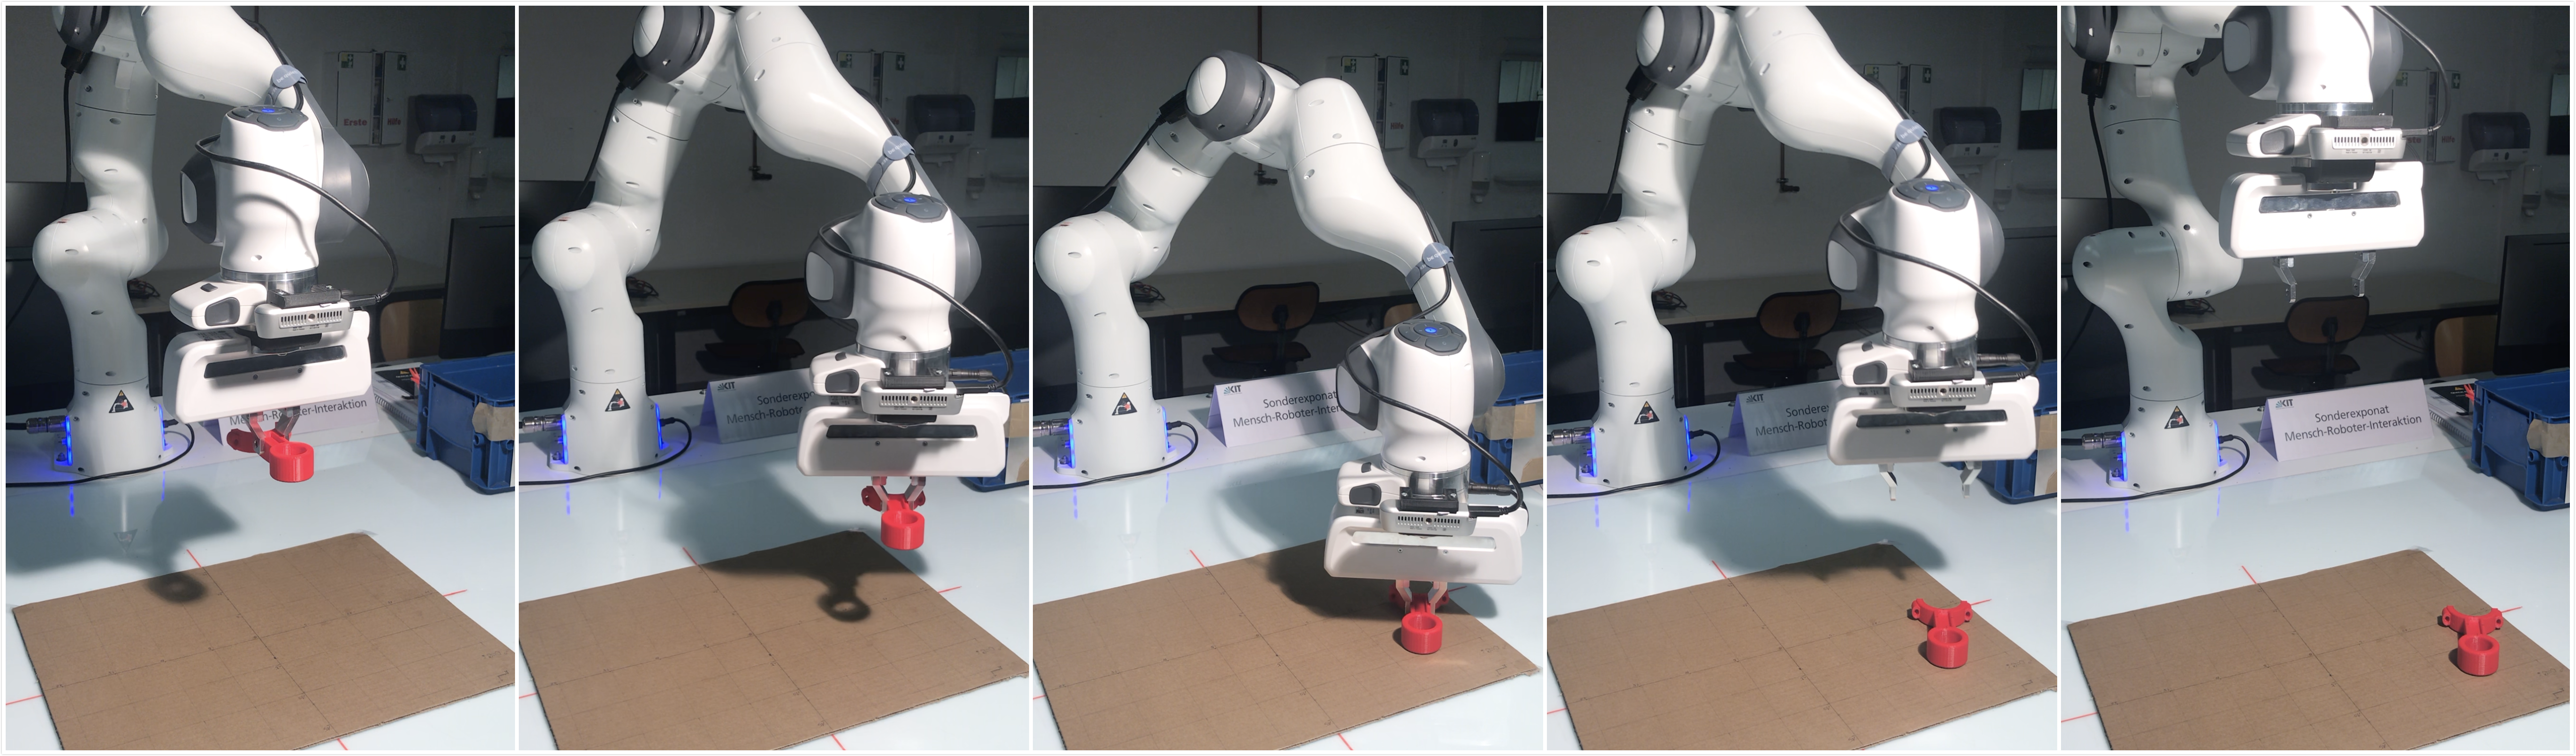
\includegraphics[width=\textwidth]{Figures/Section4_realimage.png} 
	\centering
	\caption{The process of image acquisition through the robot. The robot places the object at the target location and then returns to the camera's default position to get the image.}
	\label{fig:realimage}
\end{figure}


In the whole process, only the number of required images need to be input, and the data acquisition can be realized automatically, which simplifies the process of data collection.



